\documentclass[11pt,a4paper]{article}
% Answers to Jerome's questions of the call of 19 October 2026, and the results kept for the paper.
% Sources: experiments/registry/E51-E54.json (predictions written before each run), tools/core/read_e5*.py,
% tools/core/figures.py (prints every plotted number), docs/PAPER_CORE_2026-10-20.md (the full ledger).
\usepackage[T1]{fontenc}
\usepackage[utf8]{inputenc}
\usepackage{lmodern}
\usepackage{amsmath,amssymb}
\usepackage[margin=2.2cm]{geometry}
\usepackage{microtype}
\usepackage{booktabs}
\usepackage{graphicx}
\usepackage[font=small,labelfont=bf]{caption}
\usepackage{enumitem}
\usepackage[hidelinks]{hyperref}
\graphicspath{{figures/}}
\setlist{itemsep=0.15em,topsep=0.25em,leftmargin=1.3em}
\setlength{\parindent}{0pt}
\setlength{\parskip}{0.4em}
\renewcommand{\topfraction}{0.9}\renewcommand{\textfraction}{0.07}\renewcommand{\floatpagefraction}{0.85}

\title{\textbf{Answers to the questions of 19 October}}
\author{Giovanni Mantovani}
\date{20 October 2026}

\begin{document}
\maketitle
\vspace{-1.5em}

\section*{In short}

\begin{enumerate}
\item \textbf{The paper in three messages} (the summary figure, Figure~\ref{fig:summary}): diffusion breaks the Markov
property at intermediate times; belief propagation that knows the chain learns the exact score from few samples; it works on
the stochastic Allen--Cahn field.
\item \textbf{Temperature from a neural kernel} (Q6): for any kernel of the gradient class, the mixed second derivative of
$\log K$ is $1/\gamma$ and $-\tfrac12\log K(a\mid a)$ is the site energy. Applied to the MDN, the temperature comes back
within $10\%$ on all six cells; the potential only on the base cell.
\item \textbf{$\log Z$} (Q1) has no closed form for the quartic chain; it is computed from the top eigenvalue of the transfer
operator to $10^{-13}$, and the same solver reproduces the Gaussian closed form to $2\cdot10^{-14}$.
\item \textbf{Speciation per site} (Q8): neither an avalanche nor all at once. The bulk of a domain commits as a block; the
kinks are located last, by a short front moving from the bulk to the wall.
\end{enumerate}

Four new runs, each registered with its predictions before it ran: E51 (readings off every learned kernel), E52 ($\log Z$),
E53 (per-site polarisation), E54 (a CNN trained by standard denoising score matching on the field).

%=====================================================================================================
\section{The summary figure and data efficiency}

\begin{figure}[h]
\centering
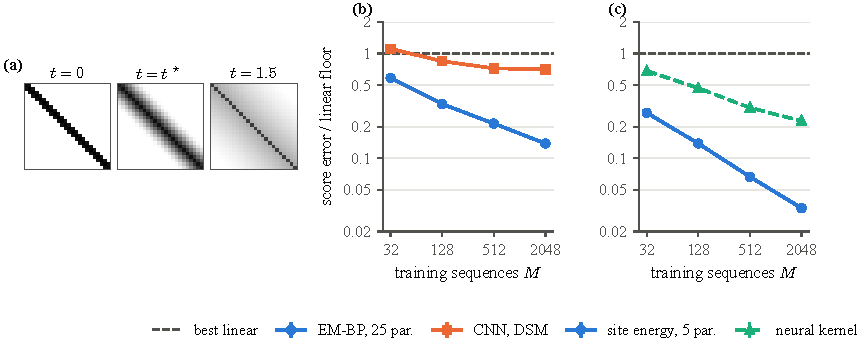
\includegraphics[width=\textwidth]{fig1-summary.pdf}
\caption{(a) $|Q_t|$, the precision matrix of the noisy Gaussian chain ($\rho=0.85$, $L=24$, log grey scale): tridiagonal at
$t=0$, densest at $t^\star\approx0.08$, nearly diagonal at $t=1.5$. (b) Laplace chain ($\rho=0.85$, $L=32$): score error of
EM--BP (mixture kernel, 25 parameters) and of a CNN trained by standard denoising score matching, divided by the best linear
estimator's, against the number of training sequences; 16 seeds, bars one standard error. (c) The same on the Allen--Cahn
field (base cell, $\Theta=0.3$, $h=1$): the 5-parameter site energy, the neural kernel inside BP (MDN, 1{,}516 parameters)
and the CNN.}
\label{fig:summary}
\end{figure}

On the Laplace chain EM--BP with $32$ sequences is more accurate than the CNN with $2{,}048$, and EM--BP with $128$ sequences
(risk $0.055$) is more accurate than the best of six network architectures with $2{,}048$ ($0.060$). The networks see the
clean sequences and fresh noise at every step; EM--BP sees one noisy copy of each sequence. On the field the site energy is
$3$--$17\%$ of the linear error at $M=2048$ on all six cells (Table~\ref{tab:field}).

%E54-TABLE

%=====================================================================================================
\section{Reading the physics off a kernel (Q5, Q6, Q7)}

\textbf{What the spline fits} (Q5). The spline kernel is $K(a'\mid a)=\mathcal N(a';a,\gamma)\,g(a')/Z(a)$: a Gaussian bond with
one free variance $\gamma$, times a free tilt $g$ of the arrival point (24 B-splines). It fits the whole pair energy, but with
the bond forced to be Gaussian. Every kernel of this form is the Gibbs chain of
\[
W(a,a')=\frac{(a'-a)^2}{2\gamma}+f(a)+f(a'),\qquad f=-\tfrac12\log(g/Z),
\]
so it is in the same class as the site-energy kernel, with more parameters.

\textbf{Two identities.} For every kernel of this class, whatever $f$,
\[
\frac{\partial^2\log K(a'\mid a)}{\partial a\,\partial a'}=\frac1\gamma,\qquad\qquad f(a)=-\tfrac12\log K(a\mid a)+\text{const}.
\]
The first holds because the terms in $a$ alone and in $a'$ alone vanish under the mixed derivative; the second because the bond
vanishes at $a'=a$. With $a=\phi/s$: $\hat\Theta=\hat\gamma s^2/h$ and $\hat V(\phi)=(2\hat\Theta/h)\hat f(\phi/s)$. On the
spline and site-energy fits these readings agree with the kernels' own parameters to $10^{-14}$; so the temperature of the spline
is read from its bond alone, and its potential from its diagonal.

\textbf{What exports to the MDN} (Q6). The identities need no parameter, so they apply to the MDN, where the mixed derivative is
no longer constant: we average it under the kernel's own stationary pair law. At $M=2048$ the MDN's $\hat\Theta/\Theta$ is
$0.91$ on the base cell and $0.97$--$1.00$ on the other five. Its potential is right on the base cell (barrier $0.20$, true
$0.25$; Figure~\ref{fig:readings}a), but off by $1.5$--$3.4\times$ on the fine and hot lattices, where the factor $2\Theta/h$
($2.4$ to $27$) multiplies the kernel's error. The spread of the mixed derivative measures how far the MDN is from the class
(coefficient of variation $0.4$--$1.0$); it does not predict the MDN's score error well (Spearman $0.24$).

\begin{figure}[h]
\centering
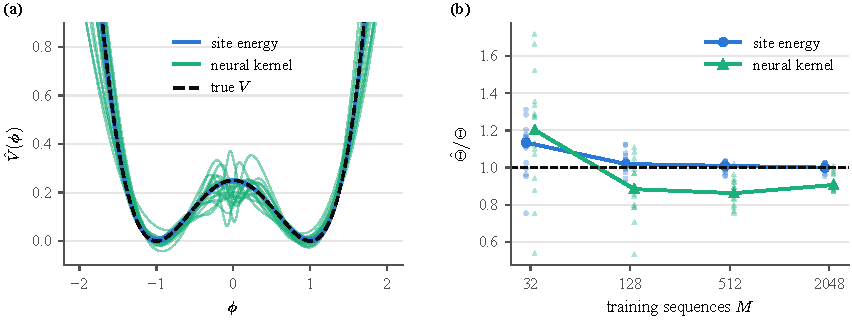
\includegraphics[width=\textwidth]{fig4-field-readings.pdf}
\caption{The physics read off kernels learned through the noise, base cell. (a) The potential from the diagonal of the
kernel, one curve per seed (16), $M=2048$: site energy and neural kernel (MDN), true double well dashed. (b) The temperature
from the mixed derivative of $\log K$, every seed a point, medians joined.}
\label{fig:readings}
\end{figure}

%=====================================================================================================
\section{Is \texorpdfstring{$\log Z$}{log Z} known? (Q1)}

For a chain of $L$ sites, $\log Z_L=L\log\lambda_0+O(1)$ and $\xi=1/\log(\lambda_0/\lambda_1)$, where $\lambda_0>\lambda_1$ are
the top eigenvalues of the transfer operator
$T(\phi,\phi')=\exp\!\big(-\tfrac{h}{2\Theta}[V(\phi)+V(\phi')]-\tfrac{(\phi'-\phi)^2}{2\Theta h}\big)$.
For a quadratic $V$ the operator is Gaussian and $\lambda_0$ is in closed form. For the quartic double well no closed form is
known: in the continuum limit the eigenproblem is the Schr\"odinger equation of the quartic double well (the transfer-integral
method of Scalapino, Sears and Ferrell, 1972; Krumhansl and Schrieffer, 1975; Khare, Habib and Saxena, 1997, note that the
$\phi^4$ case has no exact solution). So the field is an interacting model whose answer is not known in advance.

Numerically it is easy. A dense eigensolve of the trapezoid-discretised operator reproduces the Gaussian closed form to
$2\cdot10^{-14}$, and the quartic $\log\lambda_0$ changes by $2\cdot10^{-13}$ from $2401$ to $4801$ points (E52):

\begin{center}\small
\begin{tabular}{lccccccc}
\toprule
$\Theta$ ($h=1$) & 0.2 & 0.3 & 0.5 & 0.7 & 1 & 1.5 & 2 \\
\midrule
$\log\lambda_0$ per site & $-0.467$ & $-0.186$ & $0.161$ & $0.362$ & $0.550$ & $0.737$ & $0.857$ \\
$\xi$ (sites) & 19.47 & 6.08 & 2.75 & 1.98 & 1.53 & 1.21 & 1.06 \\
\bottomrule
\end{tabular}
\end{center}

As $\Theta$ falls, $\log\lambda_0$ approaches its value for a single harmonic well (the gap is $0.08$ at $\Theta=0.2$), and $\xi$
grows like $e^{E_{\rm kink}/\Theta}$ (a dilute gas of kinks; E50 fits the exponent $0.99$ against $2\sqrt2/3=0.94$).

%=====================================================================================================
\section{Speciation per site (Q8)}

We follow exact Ornstein--Uhlenbeck paths of clean chains ($L=256$, $32$ chains per temperature); read backwards, such a path
has the law of a generation with the exact score. At each of 80 levels, grid BP with the true kernel gives every site's sign
probability. A site has committed when $P(\text{correct sign}\mid x_t)\ge 0.75$ at that level and every lower one.

\begin{figure}[h]
\centering
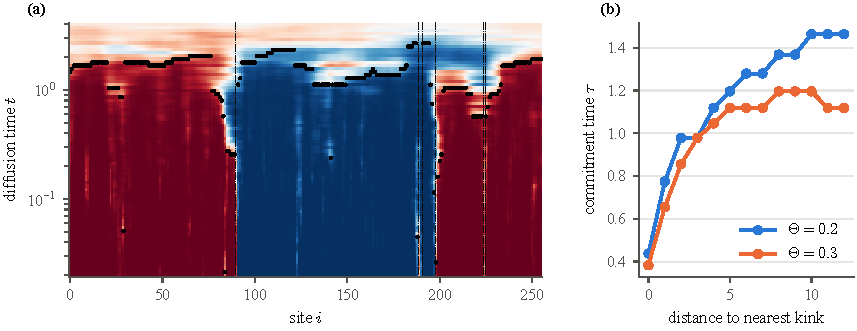
\includegraphics[width=\textwidth]{fig5-speciation.pdf}
\caption{(a) The polarisation $2P(a_i>0\mid x_t)-1$ of one chain at $\Theta=0.2$ ($\xi=19.5$ sites), red positive, blue
negative; dots: commitment times; dotted lines: the kinks of the clean chain. (b) Median commitment time against the distance
to the nearest kink, all domains of at least 8 sites.}
\label{fig:speciation}
\end{figure}

The bulk of each long domain commits as a block, at one level across tens of sites. The posterior then locates the kinks last:
the commitment time falls smoothly from $1.46$ ten sites inside a domain to $0.44$ at the kink ($\Theta=0.2$). Short domains
commit last, and a minority domain can carry its neighbour's sign for a while before it flips. Nothing propagates across a
kink. Of the three predictions registered, ``sites next to a kink commit last'' was confirmed; ``all at once inside a domain''
was falsified (the within-domain spread is $0.6$ of the spread between domains, because of the front at the walls); ``longer
domains first'' held at $\Theta=0.2$ only.

%=====================================================================================================
\section{Short answers}

\begin{description}[leftmargin=0pt,itemsep=0.35em]
\item[Why 5 parameters (Q2).] The lattice energy is a quadratic bond plus a quartic site potential, so one bond variance and a
degree-4 site energy contain the truth.
\item[Does EM see clean data (Q9).] No. EM--BP sees only the noisy sequences; the DSM networks see the clean ones in their
loss, so the comparison favours the networks.
\item[The CNN's window (Q4).] Radius 2, 4, 8 sites at $h=1,\tfrac12,\tfrac14$ (the same physical reach), chosen on development
seeds; the correlation length is about 6 sites.
\item[Is the chain directional (Q14).] No: the stationary chain is reversible, $\pi(a)K(a'\mid a)$ is symmetric.
\item[Same grid BP on the field (Q15).] Yes, 401 points on $[-8,8]$ in units of the standard deviation; 101 points give the
same risk.
\item[Gaussian messages $\Leftrightarrow$ linear score (Q10).] With Gaussian messages $\mathcal N(\mu_i,v_i)$, kernel
$\mathcal N(\rho a,q)$ and likelihood $\mathcal N(x_i;\alpha a,\Delta)$, one forward step is
\[
v_{i+1}=\rho^2\big(v_i^{-1}+\alpha^2/\Delta\big)^{-1}+q,\qquad
\mu_{i+1}=\rho\big(v_i^{-1}+\alpha^2/\Delta\big)^{-1}\big(\mu_i/v_i+\alpha x_i/\Delta\big).
\]
The variances never involve $x$ and the means are linear in $x$; the same holds backwards and for the beliefs. So
$\mathbb E[a\mid x]=Hx$ and the score is linear; on a Gaussian chain it is the exact score $-\Sigma_t^{-1}x$. Any BP whose
messages are forced to be Gaussian returns a linear estimator, at best the best linear one, which is the floor every number
here is divided by.
\item[The grid (Q11).] Figure~\ref{fig:grid}: on smooth kernels the error falls faster than any power of $N_g$ and reaches
round-off by $81$ (Gaussian) and $151$ points ($\phi^4$). On the Laplace kink it falls algebraically ($4\cdot10^{-5}$ at 201
points, $9\cdot10^{-6}$ at 401), still far below any learning error.
\end{description}

\begin{figure}[h]
\centering
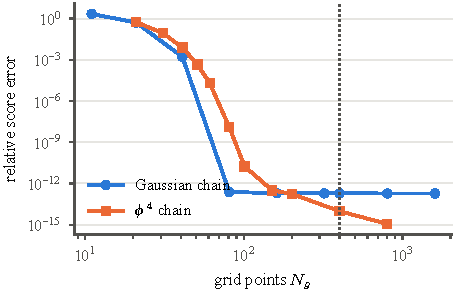
\includegraphics[width=0.48\textwidth]{fig2-grid.pdf}
\caption{Relative score error of grid BP against the number of grid points: Gaussian chain against the closed form, $\phi^4$
base cell against 1601 points. Dotted: the 401 points used everywhere.}
\label{fig:grid}
\end{figure}

%=====================================================================================================
\section{What goes in the paper}

\textbf{Body.} The summary figure; BP and the grid with its check; EM--BP, the neural kernel and the CNN against $M$ on the
Laplace chain (Figure~\ref{fig:laplace}); the same three on the field, and the temperature and potential read off the
kernels. \textbf{Appendix.} $\log Z$ and the kink gas; speciation (site-averaged and per site); the spline; the full field
table; the neural kernel off-class; oracle-free stopping; robustness across $\rho$ and $L$; cost.
\textbf{Dropped} (kept in the thesis): the Fisher/Hermite information theory, message ans\"atze and Fourier messages, the
architecture zoo and implicit score matching, the Legendre and unrestricted kernels, stride, global latent, generation,
inpainting, quench. The full list with sources is \texttt{docs/PAPER\_CORE\_2026-10-20.md}.

\begin{figure}[h]
\centering
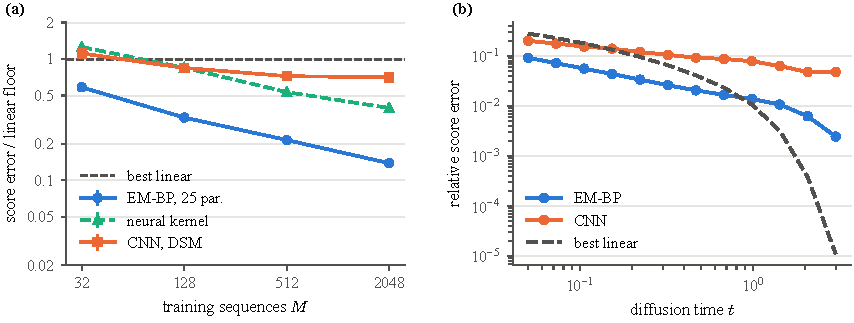
\includegraphics[width=\textwidth]{fig3-laplace.pdf}
\caption{Laplace chain. (a) The three estimators against $M$, divided by the best linear estimator. (b) Error per noise level
at $M=128$: EM--BP is below the CNN at every level; above $t\approx1$ the best linear estimator is better than both (the score
is nearly linear there).}
\label{fig:laplace}
\end{figure}

\end{document}
